%!TEX root = ../docu.tex
\section{Einleitung}

\subsection{Motivation}

Mobile Endgeräte wie Tablets und Smartphones nehmen stetig eine höhere Bedeutung im Alltag vieler Menschen ein. Dies bestätigen die aktuelle Verkaufszahlen solcher Geräte. Eine Übersicht über die Anzahl der verkauften Smartphones ist in Abbildung \ref{sale1}\cite{stat_1} dargestellt. Darin wird die seit Jahren stetig wachsende Nachfrage dargestellt, die auch im letzte Jahr einen neuen Höchststand erreichen konnte. Hervorzuheben ist, wie sich die Marktanteile der verschiedenen Plattformen über die Jahre verändert haben. Das viele Jahre als am fortschrittlichsten geltende Betriebssystem \emph{Symbian} (braun) verlor ab 2011 immer weiter an Bedeutung zu Gunsten des Siegeszugs der Android Plattform (hellblau).

\begin{figure}[h!t]
\begin{center}
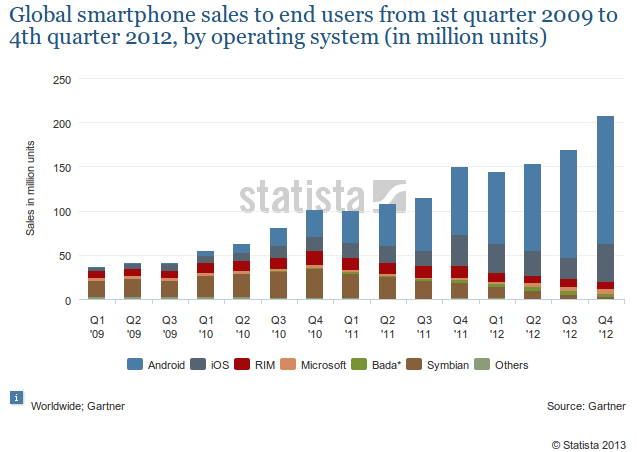
\includegraphics[scale=0.6]{images/sale}
\caption{Verkaufszahlen von Smartphones weltweit nach Plattform}
\label{sale1}
\end{center}
\end{figure}

Aktueller Vorreiter der Brache ist das auf Linux basierende Betriebssystem Android von Google Inc. Die wachsende Beliebtheit dieses Betriebssystems für Tablets und Smartphones macht es umso interessanter für Entwickler. So werden immer mehr Applikationen und Services für Geräte entwickelt, die dieses Betriebssystem nutzen. Die wachsenden Zahl an Software für Android ist in Abbildung \ref*{androidmarket}\cite{stat_2} zu erkennen. 

\begin{figure}[h!t]
\begin{center}
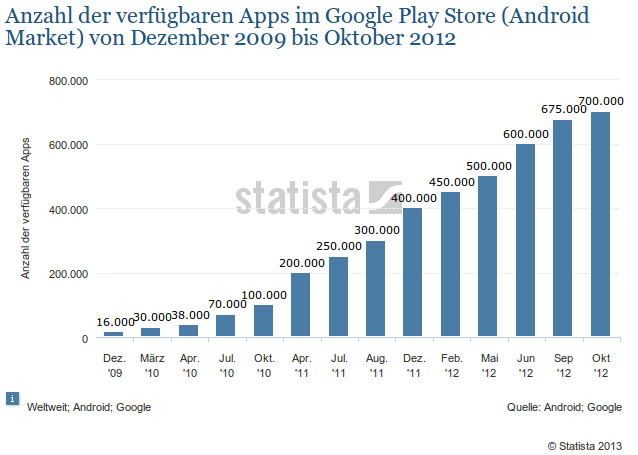
\includegraphics[scale=0.6]{images/androidmarket}
\caption{Anzahl der Applikationen für Android}
\label{androidmarket}
\end{center}
\end{figure}

Um einen Einblick in die Entwicklung von Applikationen für das mobile Betriebssystem zu bekommen, haben wir uns für die Entwicklung einer Applikation für die besagte Plattform entschieden. Diese soll für eine bestimmte Problemstellung konzipiert sein und eine angemessen Lösung darstellen.

\subsection{Vorwort}

Die Arbeit soll Einblicke in die Entwicklung von Applikationen für das Betriebssystem Android gewähren. Es werden die Grundstrukturen vorgestellt und erläutert. Diese sind nötig um die Art und Weise zu verstehen, wie Applikationen auf der Plattform ausgeführt und vom Nutzer verwendet werden können.

Abschließend werden verschiedene Probleme und Lösungswege während den Konzipierung und der Implementierung sowie während der Projektbearbeitung erläutert.

Dies beinhaltet verschiedene projektorganisatorische Elemente wie Versionierung und Projektplanung (\ref{proj}). Die folgenden Abschnitte beschäftigen sich mit der Herangehensweise an die Projektarbeit in kleinen Teams sowie deren Funktionsweise und Anwendung.

Im weiteren Verlauf werden verschiedene Schritte der Konzeptionierung sowie Implementierung verschiedener Komponentenstrukturen der Applikation diskutiert und ausgewertet. Das letztendliche Ziel der Arbeit ist eine nutzbare zweckgerichtete Applikation.

Diese Applikation soll dazu dienen die Grundlagen der Android Plattform zu verstehen. Dies beinhaltet die Funktionsweise von nativen Android Applikationen (\ref{natand}) sowie die des Android SDK. Ein tiefes Verständnis für das eigentliche Android Betriebssystem erleichtert die Entwicklung und das Verständnis über verschiedene betriebssystemspezifische Eigenheiten. Diese und weitere Grundlagen werden ebenso in dieser Arbeit behandelt und diskutiert.